\chapter{Operations in the simulated environment}
\label{cha:simworld}

\noindent\begin{wrapfigure}[16]{r}{0.3\textwidth}
    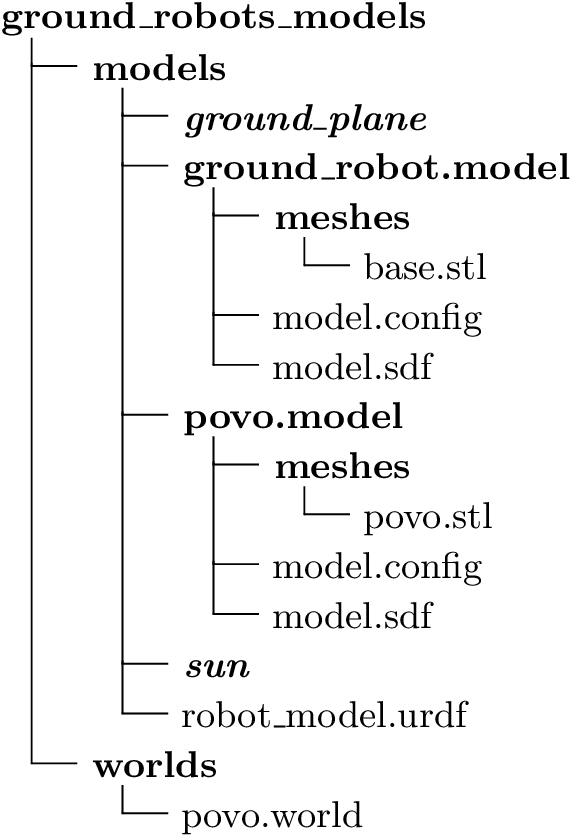
\includegraphics[width=0.3\textwidth]{images/models_folder}
    \caption{Models folder}
\end{wrapfigure}
The choice to develop a \textbf{simulation} is due to the fact that sometimes you may not physically be in university to use the real robot. The challenge here is to do a good job with \textbf{abstraction}, which means that the simulated robot and environment should be \textbf{as close as possible} to real ones. In other words, everything that used to work (i.e. navigation and planning) should now continue to work even if you are no longer in the real world; in theory you should not notice if you are in the real world or in a simulated one.

\section{Models}

To get a complete simulation, we need to create what is missing from reality, which environment and robot models.

\subsection{Environment}
\label{sub:map}

A mesh of the upper floors of Povo was provided by Professor \textit{Marco Roveri}\cite{roveri}. Unfortunately, compared to the navigation map generated by real data, it turns out that the mesh is \textbf{not very accurate}. Two workarounds are possible: create a \textbf{new navigation map} for simulation purposes or \textbf{adapt the mesh} to the real environment with some modifications; it turns out, as described in \autoref{sub:waypoints}, that already only by scaling up one side of the mesh, you get a better result. 

A model is then created using \acrfull{sdf} and later inserted inside a \code{world} file\footnote{A collection of the models you want to display in the Gazebo scene, always written in \acrshort{sdf}}.

\bigskip

\begin{figure}[h]
    \centering
    \includegraphics[width=0.8\textwidth]{images/3d\_povo\_model}
    \caption{Povo model for simulation. Colors were used for a better visualization.}
\end{figure}

\subsection{Robot}
\label{sub:robot}

Part of the setup is inspired to \textit{Automatic Addison} tutorials\cite{tutorials}.

The robot mesh was created starting from the \textit{shelfino} shape (see \autoref{fig:shelfino}), trying to keep it \textbf{as similar as possible}, and each piece (robot base, lidar, wheels and caster wheel) was exported singularly. For performance reasons in Gazebo, the only mesh actually used is the robot base, because of its special structure to \textbf{avoid contact} with the wheels \textbf{partially inside}. The other ones are replaced by \acrshort{sdf} or \acrfull{urdf} built-in geometric shapes (i.e. cylinders).
Both \acrshort{sdf} and \acrshort{urdf} files have been used: the first one for Gazebo and the second one for a node called \code{robot\_state\_publisher} that helps to visualize the robot in \acrshort{rviz}.

\begin{figure}[h]
    \centering
    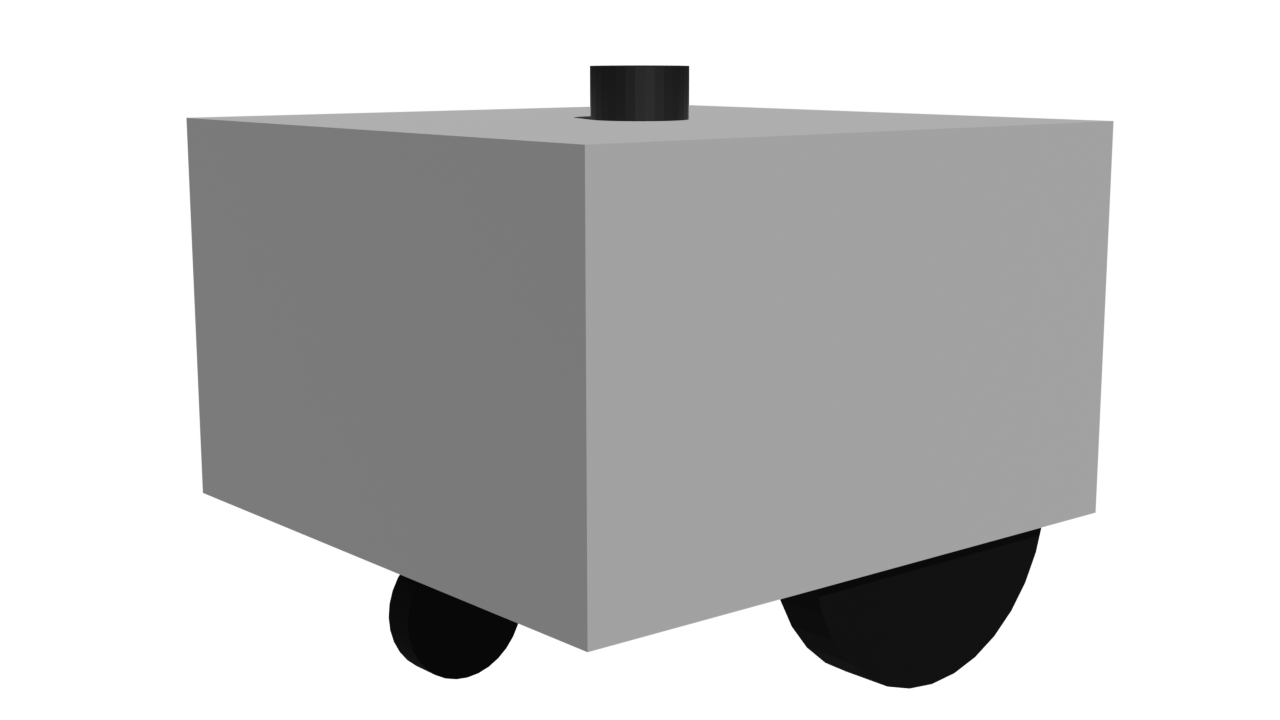
\includegraphics[width=0.7\textwidth]{images/shelfino_3d.png}
    \caption{Shelfino model for simulation.}
\end{figure}

\section{Gazebo plugins}

After placing the models in Gazebo, we need a way for our robot \textbf{interact} to interact with the environment. You can no longer utilize the nodes in \autoref{subsec:nodes} because they make use of a real hardware, but thankfully Gazebo provides some \textbf{plugins} that can be added to the \acrshort{sdf} model as a normal tag. We always need a way to set the \textbf{linear and angular velocities} to make the robot moves as desired, a way to \textbf{calculate odometry} and a lidar to \textbf{detect obstacles}. Once done, the robot can be used as if it were a real robot.

Sadly, there are no plugins available for tracking cameras, so we content ourselves with only wheels rotation information to calculate odometry. 

\subsection{Differential drive plugin}

It brings differential drive controls to the simulation; after setting the names of wheel joints and their properties, such as the wheels separation and diameter, it allows you to control its velocity over \code{cmd\_vel} topic and see its position and rotation in the space over the \code{odom} topic and transformation.

\subsection{Ray sensor plugin}

To allow the robot to able to detect obstacles, a lidar is required. To do so, you can simpy use the Gazebo \textbf{sensor} \code{ray} tag, setting \textbf{scan}, \textbf{range} and \textbf{noise} information, but even a plugin is required to make it work. The only necessary configurations are:
\begin{itemize}
    \item which \acrshort{ros} message type to use as \textbf{output} (\code{sensor\_msgs/LaserScan});
    \item frame name to which the lidar is \textbf{attacched} (described elsewhere else in the model).
\end{itemize}